\section{``Get a Good Ball to Hit'' -Rogers Hornsby}
In 1971 left-handed hitter Ted Williams published what many baseball players consider a bible of their craft,``The Science of Hitting'' \citep{Williams1971}. In it, Williams credits baseball legend Rogers Hornsby for unsurpassed advice: ``Get a good ball to hit.''
        \begin{figure}[H]
      	\centering
      	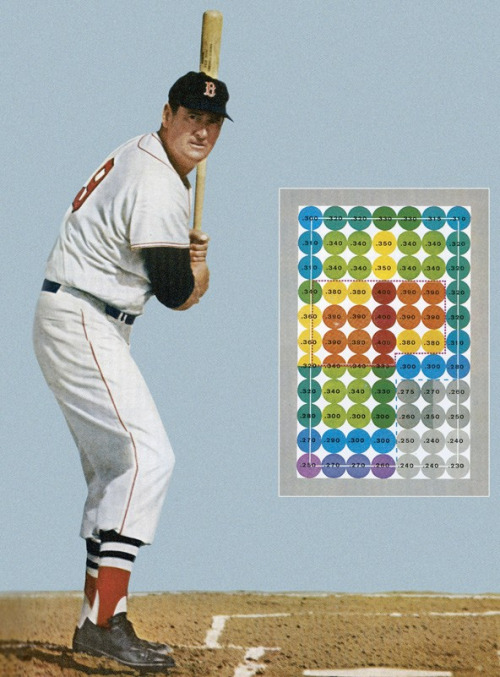
\includegraphics[scale=.29]{Images/Williams.jpg} 
      	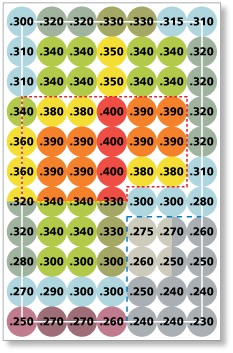
\includegraphics[scale=0.55]{Images/SZ.jpg}
      	\caption{Ted Williams conceptualized the strike zone as divided into pitch locations, with specific probabilities of getting a hit. In this iconic image he labeled the baseballs with his own estimated batting average on pitches in that location \citep{Williams1971}.}
      	\end{figure} 
Horsby meant that location makes some pitches easier to hit than others, and  Williams's famous strike zone visual in Figure 1 encapsulates this advice\footnote{Please see Appendix A for baseball background information, rules and workings; or \citep{Wiki}}. Prior to 2008, no data existed to analyze, visualize, and model William's location-based conception of the stike zone. However, in 2008 MLB collaborated with Sportsvision, to implement a new technology called PITCHf/x\textsuperscript{\textregistered}, which collects the necessary data for such an analysis.

\section{The Data} % ============================================
Sportvision, Inc., a company based in Chicago, provides the technology to collect PITCHf/x\textsuperscript{\textregistered} data. In 2007 and 2008 Sportvision installed two high speed stereoscopic cameras in every MLB\textsuperscript{\textregistered} stadium. These cameras take 20 images of each pitch in flight and determine its 3-D path \citep{Fast2010}. Sportsvision licenses PITCHf/x\textsuperscript{\textregistered} data to Major League Baseball Advanced Media (MLBAM\textsuperscript{\textregistered}) \citep{Baumer2010}. 

MLBAM\textsuperscript{\textregistered} makes PITCHf/x\textsuperscript{\textregistered} data publicly available online in XML format, calling it ``Gameday'' data \citep{Sievert2014}. A homepage exists for every game, with links organizing data into XML tables such as game, inning, at bat, pitch, team, player, and umpire \citep{Sievert2014}. The at bat table, for example, contains 15 variables for 1,711,211 at bats. The format and size (on the order of gigabytes) of the data precludes direct download impractical. Instead, XML scripts automate database ready downloads \citep{Adler2006}. We used the MySQL database management system to manipulate and store 13 PITCHf/x\textsuperscript{\textregistered} tables \citep{Tahaghoghi2006}. 

R, an ``{\it in-memory} application,'' uses a computer's limited RAM to host the R environment data \citep{Smith2013}. As a result, data manipulation on this scale requires ``memory management'' techniques \citep{Wickham2014}.  We applied Split-Apply-Combine operations to tables inside the MySQL database, before importing data frames to R \citep{Wickham2011}.

We collected the variables relevant for this research predominantly from the `at bat' and `pitches' tables. These variables, with a short description, follow \citep{Fast2007}.
  \begin{itemize}
  \item \verb|px| - location of the pitch on the horizontal axis when it passes through the strike zone (or the extended plane). \verb|px| is recorded in feet from the middle of home plate, from the catcher/umpire point of view.
  \item \verb|pz| - location of the pitch on the vertical axis when it passes through the strike zone plane, measured in feet above the ground. A negative value implies the ball bounced before reaching home plate
  \item \verb|des| - a short description of the outcome of the pitch, i.e. swing and miss, ground ball for out, ground ball for hit, etc.  
  \item \verb|id| - a unique id for a pitch within a game
  \item \verb|ab_id| - a unique id for each at bat  
  \item \verb|pitch_id| - a unique identification number for each pitch
  \item \verb|pitch_type| - a classification of the type of pitch, out of 18 possible types. For example, four seam fastball, two seam fastball, curveball, knuckle ball, etc.
  \item \verb|stand| - handedness of the batter; right or left.
  \item \verb|batter| - a unique ID for each hitter
  \end{itemize}

% The variable \verb|des|, short for `description,' describes pitch outcomes. In this study, we use swing outcomes described in \verb|des| to define a Bernoulli random variable $S$ (Section 3.1) that equals one for a hit, and equals zero for {\it any} swing that does not result in a hit. This modifies the current standard, where analyses include only swings that end at bats \citep{Cross2015}, \citep{Baumer2010}, \citep{Fast2011}. We submit that {\it every} swing represents a trial, and failure to get a hit should be evaluated separately from the count in the at bat at the time of the trial.

\section{Research Significance to Professional Baseball Organizations and Media}

Major League Baseball (MLB\textsuperscript{\textregistered}) teams exploy approximately 156 quantitative analysts, at a total cost of approximately \$15 million annually \citep{Lindbergh2016}. Teams strive to gain marginal competitive advantages, so novel modeling and analysis of strike zone data could generate substantial interest. For example, results indicate hitters have higher success probabilities in the lower 1/3 of the strike zone than in the top 1/3, but this contradicts conventional wisdom advising pitchers to ``keep the ball down'' \citep{Stallings2003}. An interpretable model that explains why this is bad advice may change minds. As a second example, if these interpretations are in biomechanical language, biomechanists may analyze the relationships between body types and spatial success probabilities. This could in turn help MLB\textsuperscript{\textregistered} team scouting departments more accurately preduct hitting success for amateur players, a notorously difficult but lucrative challenge. For a final example, some MLB\textsuperscript{\textregistered} players, such as Joey Votto, have a keen interest in using the most sophisticated analytics available to understand the keys to their success and failure\citep{Daugherty2015}. This research would fit that criteria for Votto.

With regard to media usage possibilities, heat maps are frequently included in television broadcasts of MLB\textsuperscript{\textregistered} games \citep{Cross2015}. ESPN\textsuperscript{\textregistered} and MLB\textsuperscript{\textregistered} recently agreed to an eight year, \$5.6 billion contract \citep{Newman2012}; cutting-edge, more informative heat maps would improve the quality of game broadcasts.

As the dollar amounts indicate, it is not for a lack of motivation that the research questions posed here remain open. Rather, the solutions require an array of statistical and computational competencies. In addition, the data are quite new, and relatively inaccessible without data management and programming skills.

% The methods we will use for addressing these questions will include and integrate generalized linear models \citep{Myers2012}, spatial statistics \citep{Oliver2005}, and Bayesian hierarchical models \citep{Gelman2014}. We will employ these methodologies using the statistical software R \citep{R2015}, the Bayesian statistical software and programming language Stan \citep{Gelman2015}, the R to Stan interface RStan \citep{RSTAN}, advanced data visualization tools in ggplot2 \citep{Wickham2009}, baseball specific programming techniques \citep{Marchi2013}, and the open-source Relational Database Management System (RDMS) MySQL \citep{Tahaghoghi2006} for storing and managing a 1.82 GB (to date) PITCHf/x\textsuperscript{\textregistered} database.


\section{Statistical Research Contributions and Context}

This research includes novel applications of advanced, cutting edge statistical techniques. In addition, as of publication, only one article in a peer reviewed journal focuses on this area of application. This combination---novel application of existing techniques to an unstudied area---constitutes a significant statistical research contribution. 

The area of application is, of course, baseball. More specifically, we analyze strike zone data. As of publication, \cite{Cross2015} constitutes the only baseball statistical analysis article in a peer reviewed journal. This is surprising, given the widespread enthusiam for baseball, until considering the obstacles. Perhaps most importantly, data collection began relatively recently, in 2008. Further, an individual must possess advanced statistical training, programming abilities, database management skills, and baseball interest. The intersection of these subsets of people proves quite small!  Together, these factors explain the paucity of research.

Our efforts build on others' work, and in some cases stand on the shoulders of giants. Our inspiration to model strike zone success owes \cite{Williams1971} a debt, and \cite{Cross2015} provided a place in the literature to start. However, we sought a paremetric parametric model, and logistic refression fit the bill \citep{Myers2012}. The initial heat map in \cite{Cross2015} intimated polar coordinates could be a key. Thinking of pitch locations, in polar coordinates, as biomechanical covariates was perhaps inspired by the works of, and conversations with, Glenn Fleisig at the American Sports Medical Institute \citep{Fleisig2002}, and Brittany Dowling of Motus \citep{Dowling2016}. \cite{Hosmer2013} provided such logistic regression models an early proof of concept. From there, two  paths emerged; (i) visualizing our data and analysis, and (ii) the "big N" problem.

Our empirical heat maps provided the opportunity for innovation, and Hadley Wickham's \verb|ggplot2|, and its ``layered grammar of (\verb|ggplot2|) graphics,'' was our palette \citep{Wickham2009}, \citep{Wickham2010}. Unseen but integral, the spatial data package \verb|fields|, created by a colleague Doug Nychka at NCAR, provided a kind of computational mortar in these efforts.  In addition, we saw the need for improved heat map CIs, and RStudio's Shiny, an ``interactive web application framework,'' offered the necessary tools \citep{Shiny}.

In the Bayesian paradigm it seemed relatively simple at first to add a spatial random effect to a generalized linear model, giving a bayesian hierarchical spatial model \citep{Gelman2014}, \citep{Banerjee2014}. However, the "big N" problem required numerous shoulder resources to stand on. The first shoulders were familiar; Hadley's \verb|dplyr| was indispensable \citep{Wickham2016}. The ``split-apply-combine strategy,'' in tandom with MySQL, proved critical for data wrangling \citep{Wickham2016}, \citep{Tahaghoghi2006}. This really only got us started though. Attempting to computationally and statistically deal with the ``big N'' problem involved three general approaches: (i) computational optimization, (ii) dimension reduction, and (iii) approximation.

Our attempts at computational optimization occurred with the Bayesian programming language Stan, and the R interface \verb|rstan| \citep{rstan}, \citep{Gelman2015}. Poring over the manual  helped \citep{STANtheMan}; and so did subset of Stan developers---including Andrew Gelman, Rob Trangucci, and Bob Carpenter.

The second approach, dimension reduction, came from colleague Andrew Finley's work, in Michigan State's Department of Forrestry and Geography. He played a central role in creating predictive process models, and the implementation package \verb|spBayes| \citep{Banerjee2008}, \citep{Finley2012}, \citep{Finley2013}.

Finally, we explored approximation techniques. The integrated nested laplace approximation (INLA), a mathematically and computationally complex procedures, gives speedy estimates for a certain class of models \citep{Rue2009}. However, modifying our setup to prepare for INLA required a stochastic partial differential equation \citep{Lindgren2011}, \citep{Lindstrom2016}. 

As this overview demonstrates, this work builds on the contributions of numerous other scientists and statisticians. Next, we lay out how this dissertation proceeds.


\section{Research and Literature Overview}

\section{Roadmap}

% Using PITCHf/x\textsuperscript{\textregistered} data, amateur statisticians have conducted exploratory data analysis of the spatial, hitter success, strike zone data. However, there have been virtually no publicly available\footnote{Presumably proprietary approaches by MLB\textsuperscript{\textregistered} teams exist.} professional or academic attempts to model and understand the spatial process with advanced statistical techniques. 

Chapter 2 explores the problem of resolution selection for empirical heat maps, especially those with spatially varying data density. We provide a new option for addressing this problem: variable-resolution heat maps. Two parts comprise Chapter 3. In the first part we create a generalized linear model for spatial hitter success probabilities, using biomechanical covariates. In the second part we explain the conundrum of heat map confidence intervals, and the current best practices. We provide, we believe, a better option with an interactive Shiny application \citep{Shiny}. In Chapter 3 we add a spatial random effect to the Chapter 2 model, and deal with the computational consequences. We define the ``Big N'' problem, and explore three approaches to fitting a ``Big N'' spatial generalized linear mixed model. 
